% Overview:
%   DiscoSNP++ TeX subfile for the project.
%   Each subfile MUST start with the following line
%		\documentclass[../main.tex]{subfiles}

\documentclass[../main.tex]{subfiles}

\begin{document}

\subsection{DiscoSnp\texttt{++}}
\label{discosnp++}

DiscoSnp\texttt{++} \cite{peterlongo2017discosnp++} rientra nella categoria dei metodi \textit{de-novo}, ed è stato presentato come la nuova versione di \textsc{DiscoSnp} \cite{uricaru2015reference}, framework che si proponeva di individuare SNP isolati eterozigoti e omozigoti. DiscoSnp\texttt{++} è stato reimplementato da zero usando la libreria GATB \cite{drezen2014gatb} e permette di ottenere un tempo di esecuzione più veloce ed un minor consumo di memoria rispetto alla sua precedente versione. È stato progettato per individuare e classificare tutte le tipologie di SNP, compresi piccoli indel provenienti direttamente dalle read sequenziate (FastQ\footnote{FastQ :  formato di puro testo in codice ASCII facilmente leggibile, pensato dal Wellcome Sanger Institute per associare ad una sequenza prodotta da una tecnologia HTS/NGS, la qualità di ogni sua singola base. È diventato lo standard de facto per la condivisione di dati \cite{cock2010sanger}) prodotti da processi di sequenziamento basati su tecnologia HTS. } o FASTA) senza utilizzare un genoma di riferimento, differentemente da \textsc{DiscoSnp} che era specializzato nella classificazione di una sola tipologia di SNP.

Per ottenere questo risultato DiscoSnp\texttt{++} migliora gli algoritmi presentati da \textsc{DiscoSnp} basati

\noindent
Normalmente DiscoSnp\texttt{++} restituisce gli SNP individuati e classificati nel formato VCF, ma opzionalmente può restituirli dopo averli mappati su un genoma di riferimento. Questo può inizialmente apparire in contrasto con un approccio reference free, tuttavia torna particolarmente utile quando si dispone di un genoma di riferimento che non può essere usato per effettuare la chiamata delle varianti (\textbf{variant calling}) tramite tecniche di mappatura ma che può essere usato per posizionare le varianti predette tramite tecniche de-novo. In situazione abbastanza comuni, queste casistiche si presentano quando il genoma di riferimento è stato assemblato male o si sta analizzando un genoma molto distante dalla specie sequenziata. In ogni caso, anche se ci fosse un buon genoma di riferimento, la predizione delle varianti e la genotipizzazione con l'approccio reference free non è influenzato in alcun modo dagli alleli di riferimento.

\subsubsection{Una struttura dati per identificare varianti : il grafo di \textit{de Bruijn}}
\label{dBG}

I grafi di \textit{de Bruijn} sono la struttura dati su cui si basano la maggior parte dei tool \textit{reference free} per la  ricerca di mutazioni (SNP) senza l'utilizzo dell'allinemento, in quanto eliminano la necessità di un genoma di riferimento e utilizzano direttamente i confronti della sequenza grezza.

\theoremstyle{definition}
\begin{definition} 
Dato un insieme di stringhe $S = \{r_1 , r_2 , ... , r_n\}$ su un alfabeto $\Sigma$ ed un intero $k\geq2$, il grafo di \textit{de Bruijn} di ordine $k$ di $S$ $(dBG_k (S))$ è un grafo diretto (o digrafo) $(V,A)$ dove:
\begin{itemize}
\item[-] $V = \{d \in \Sigma^k \ |\  \exists i \in \{1, ..., n\} \ tale\ che\ d\ \grave{e}\ una\ sottostringa\ di\ r_i \in S\}$
\item[-]$A = \{ (d,d^\prime)\ |\ se\ il\ suffisso\ di\ lunghezza\ k-1\ di\ d\ \grave{e}\ prefisso\ di\ d^\prime\}$
\end{itemize}
\end{definition}

\noindent
I grafi di \textit{de Bruijn} sono quindi grafi diretti che ben si adattano a rappresentare relazioni ordinate tra sequenze della stessa lunghezza, come (\textit{k}-mer) delle read (vedi Figura \ref{fig:dBG}), hanno inoltre dimostrato di essere di grande utilit\`a come modello di dati e su di esso sono stati implementati quasi tutti gli algoritmi di assemblaggio \textit{de novo} progettati per utilizzare dati provenienti da \textit{short reads}. Alcuni esempi degni di nota di questi algoritmi sono Velvet e ABySS. Nella maggior parte di questi strumenti di assemblaggio, il grafo di \textit{de Bruijn} \`e implementato come una struttura dati interna che rappresenta una rete in cui i nodi contengono i \textit{k}-mer delle read e i gli archi contengono i $k-1$ nucleotidi sovrapposti tra i \textit{k}-mers\footnote{\ Dipendentemente dalla definizione con cui si costruisce il grafo di \textit{de Bruijn}, il \textit{k}-mer pu\`o essere il nodo o l'arco che congiunge due nodi. \textbf{Definizione nodo-centrica}: i nodi sono tutte le sottostringhe di lunghezza \textit{k} di ogni stringa in $S$. Un arco $s_1 \rightarrow s_2$ è presente se il suffisso di lunghezza $k-1$ di $s_1$ è anche un prefisso di $s_2$. \textbf{Definizione arco-centrica}: tra i $k^\prime$-mer (nodi), un arco $s_1 \rightarrow s_2$ è presente se esiste un $(k^\prime+1)$-mer in una stringa di $S$ che contiene $s_1$ come prefisso e $s_2$ come suffisso. Le definizioni nodo-centriche e arco-centriche sono essenzialmente equivalenti quando $k^\prime = k-1$ (anche se nella prima i nodi hanno lunghezza \textit{k} e $k - 1$ nella seconda).\\}. In una situazione senza errori di lettura e con \textit{k} abbastanza lungo da includere la ripetizione più lunga in un singolo k-mer, \`e teoricamente possibile ricostruire il genoma seguendo il cammino formato dagli archi che congiungono tutti i \textit{k}-mer, passando attraverso ogni \textit{k}-mer solo una volta. 

\begin{figure}[h!]
	\centering
  	\captionsetup{justification=centering}
  	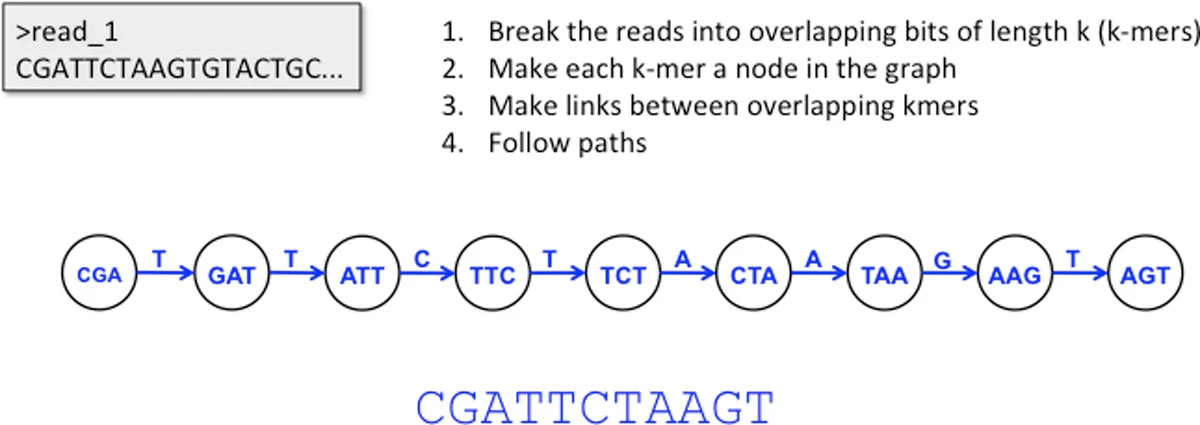
\includegraphics[scale=.3]{images/dBG.png}
  	\caption{Esempio di grafo di \textit{de Bruijn} costruito da k-mers sovrapposti.}
  	\label{fig:dBG}
\end{figure}

\noindent
Poich\`e i dati sequenziati contengono errori (stimati tra lo 0.1\% e l\textquotesingle 1\%) e le ripetizioni genomiche possono essere molto lunghe, gli errori sulle read possono causare vicoli ciechi nel percorso e ripetizioni nel genoma puossono causare cicli nel grafo. Una mutazione (SNP) causerà con alta probabilità queste sottostrutture. Perci\`o concentrandoci su queste strutture, anzich\`e buttarle via, si possono identificare la variazioni direttamente all\textquotesingle interno del grafo. La struttura di base che indica la presenza di un SNP è descritta come una `bolla' (vedi Figura \ref{fig:dBG_bubble}).

\begin{definition}
Una bolla \`e una biforcazione chiusa di un cammino ed \`e causata da una singola differenza nucleoditica alla fine di un \textit{k}-mer. Partendo da un nodo (sinistro) chiamato \textit{start} \`e possibile seguire i cammini generati dai due nodi figli $n_h$ e $n_l$ (rispettivamente chiamati \textit{superiore} e \textit{inferiore}) terminando in un nodo (destro) chiamato \textit{end}. Dipendentemente dal tipo di mutazione (SNP) che ha prodotto la bolla, i due cammini possono avere lunghezze diverse. Se il nodo \textit{start} ha più di due nodi figli (destri), tutte le possibili coppie sono trattate come $n_h$ e $n_l$.
\end{definition}

\begin{figure}[h!]
	\centering
  	\captionsetup{justification=centering}
  	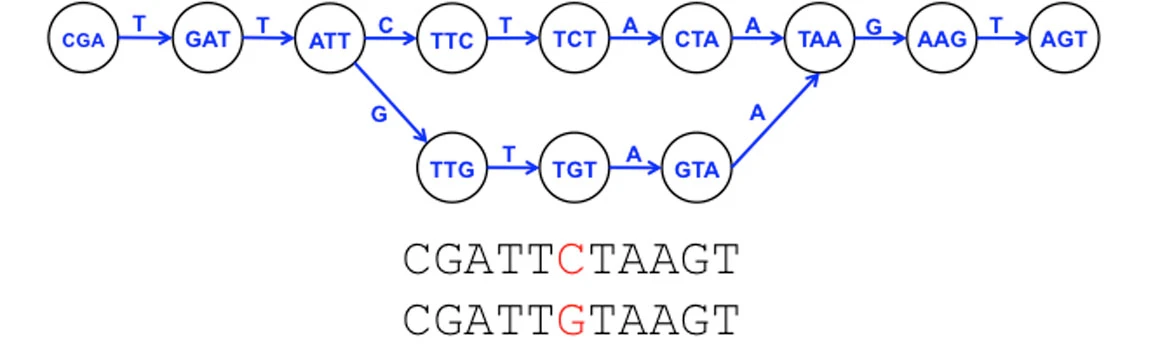
\includegraphics[scale=.3]{images/dBG_bubble.png}
  	\caption{Esempio di bolla all'interno di un grafo di \textit{de Bruijn}.}
  	\label{fig:dBG_bubble}
\end{figure}

\paragraph{Strategie per identificare variazioni} \`E ormai chiaro che l\textquotesingle analisi delle bolle all\textquotesingle interno di un grafo di \textit{de Bruijn} risulta cruciale per riuscire a comprenderne il loro contenuto informativo. In letteratura, \cite{leggett2014reference} presenta alcune strategie per identificare le mutazioni. \\ \textcolor{red}{Secondo te ha senso questo sotto paragrafetto? Parlerei delle tecniche quindi: Depth-first, Topological, Microassembly, Maximum Likelihood Methods, Contig based Graph.}

%In quanto la ricostruzione di una sequenza di input equivale alla ricerca di un cammino hamiltoniano\footnote{\ Un cammino in un grafo (orientato o non orientato) è detto \textbf{hamiltoniano} se esso tocca tutti i vertici (nodi) del grafo una e una sola volta. Determinare se questo cammino esista è un problema NP-completo. Un grafo che contiene almeno un ciclo hamiltoniano è detto \textbf{grafo hamiltoniano}.} all'interno del grafo, noto problema NP-completo.


\subsubsection{Struttura dati di DiscoSnp\texttt{++}}

DiscoSnp\texttt{++} basa la sua efficienza sulla struttura dati Minia \cite{chikhi2013space} che permette di costruire grafi di \textit{Bruijn} probabilistici. Questa specifica struttura dati è ottenuta inserendo tutti i nodi di un grafo di \textit{Bruijn} classico all'interno di Bloom Filter posti in cascata. All'interno di questa struttura dati, differentemente da un grafo di \textit{Bruijn} classico, gli archi sono dedotti implicitamente dalle interrogazioni fatte ai Bloom Filter per l'appartenenza di tutte le possibili estensioni di un \textit{k}-mer e non necessitano di essere memorizzati. In particolare, un'estensione di un \textit{k}-mer \textit{v} è la concatenazione di un suffisso $\textit{k}-1$ di \textit{v} con uno dei quattro possibili nucleotidi o di uno dei quattro nucleotidi con il prefisso  $\textit{k}-1$ di \textit{v}. \textcolor{red}{Minia inoltre supporta un conteggio efficiente ed esatto dei vicini di qualsiasi nodo nel grafo. Pertanto, questo consente di attraversare in modo efficiente il grafo a partire da qualsiasi nodo, in entrambe le direzioni.}


Quindi riuscire ad ottimizzare la ricerca all'interno questa struttura dati è quello che si propone DiscoSnp\texttt{++} tramite i $dBG$ \textit{probabilistici}.\\

\subsubsection{Algoritmo di DiscoSnp\texttt{++}}

\paragraph{} Gli algoritmi presenti all'interno dei moduli di \textsc{DiscoSnp} (\textsc{KisSnp2} e \textsc{KissReads}) sono stati stati rivisitati per ottenere un miglior filtraggio degli errori di sequenziamento in modo da individuare nuove mutazioni (SNP). 

\paragraph{}
L'algoritmo su cui si basa DiscoSnp\texttt{++}, dopo che il $dBG$ è stato costruito, si concentra sulla ricerca e la classificazione delle bolle all'interno del grafo, ovvero la ricerca di due path distinti formati da $k+2$ nodi, che hanno in comune i \textit{nodi di diramazione}\footnote{Un nodo di diramazione, o \textit{branching node}, un nodo che ha più di un predecessore e/o più di un successore.}. Tenendo conto anche del fatto che una bolla può essere o meno ramificata\footnote{Una bolla si dice \textit{ramificata} quando almeno uno dei due path contiene un \textit{branching node}. Sono esclusi da questa caratterizzazione il primo e l'ultimo nodo della bolla.}, e presentare simmetria\footnote{Una bolla ramificata può essere \textit{simmetrica} o \textit{non simmetrica}. Intuitivamente le bolle ramificate sono bolle in cui dai nodi $n_h$ e $n_l$, più di due cammini possono essere percorsi simultaneamente. Al contrario nelle bolle ramificate non simmetriche, dai nodi $n_h$ e $n_l$ esistono esattamente un unico paio di cammini (superiore e inferiore) che convergono ad un branching node di destinazione.}. Dipendentemente dai parametri DiscoSnp\texttt{++} può individuare solo bolle ramificate, o bolle non ramificate e non simmetriche, o qualunque tipo di bolla senza restizioni.

Dipendentemente dalle mutazioni (SNP), l'algoritmo classifica le bolle nei seguenti modi. Se i cammini $n_h$ e $n_l$ sono composti da esattamente $k$ nodi, allora si tratta di una mutazione (variazione) \textit{isolata} in quanto non esistono altri polimorfismi (mutazioni), e quindi \textit{branching node}, nei $k$ nucleotidi prima e dopo la posizione della mutazione. Se invece la bolla generata presenta due cammini con lo stesso numero di nodi, maggiore di $k$, siamo in presenza di una variazone \textit{non isolata}. Nel caso i cammini generati da $n_h$ e $n_l$ si presentano con un diverso numero di nodi, siamo in presenza di indel. Solitamente il cammino di lunghezza minima prodotto ha esattamente $k-1$ nodi, ma dipendentemente dal contesto in cui si verifica la lunghezza può variare ed essere inferiore a $k-1$\footnote{Accade quando l'indel e ciò che lo segue (o precede) hanno un prefisso (o suffisso) comune di dimensione $> 0$. Più precisamente se le dimensioni di prefisso e suffisso sono rispettivamente $p_1$ e $p_2$, il cammino di lunghezza minima è composto da $max(0, k-1-p_1 - p_2)$ nodi e quello di lunghezza massima è composto da $k-1+d-p_1 - p_2$ con $d$ dimensione dell'indel.}.

\begin{definition}
Una bolla \`e un cammino che partendo da un nodo di diramazione\footnote{Un nodo di diramazione, o \textit{branching node}, un nodo che ha più di un predecessore e/o più di un successore.} (sinistro) chiamato \textit{start} e seguendo i cammini generati dai due nodi figli $n_h$ e $n_l$ (rispettivamente chiamati \textit{superiore} e \textit{inferiore}) termina in un nodo di diramazione destro. Dipendentemente dal tipo di mutazione (SNP) che ha prodotto la bolla, i due cammini possono avere lunghezze diverse. Se il nodo \textit{start} ha più di due nodi figli (destri), tutte le possibili coppie sono trattate come $n_h$ e $n_l$.
\end{definition}

\textcolor{red}{Continuare qui!}

\begin{figure}[ht]
\begin{subfigure}{.5\textwidth}
  \centering
  %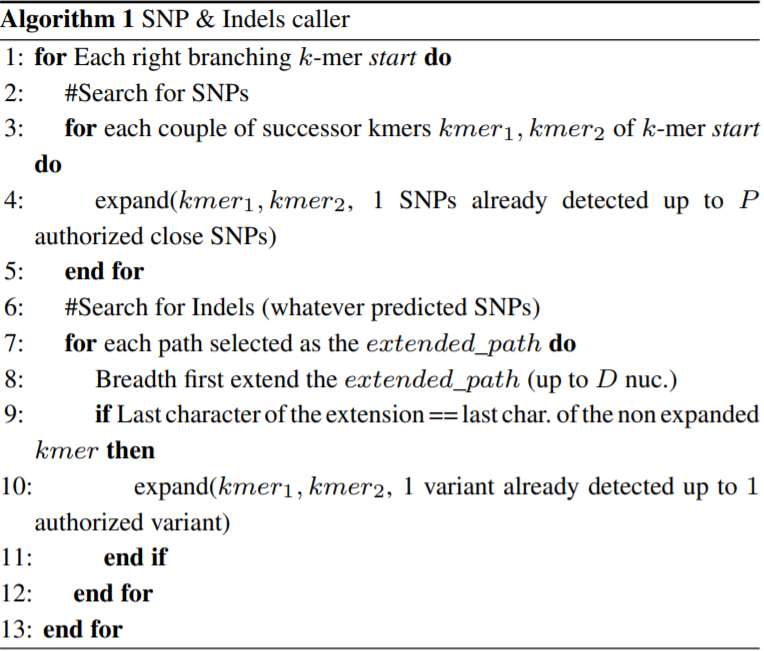
\includegraphics[width=.8\linewidth]{images/discosnp_alg1.png}
  \caption{1a}
  \label{fig:sfig1}
\end{subfigure}
\begin{subfigure}{.5\textwidth}
  \centering
 % 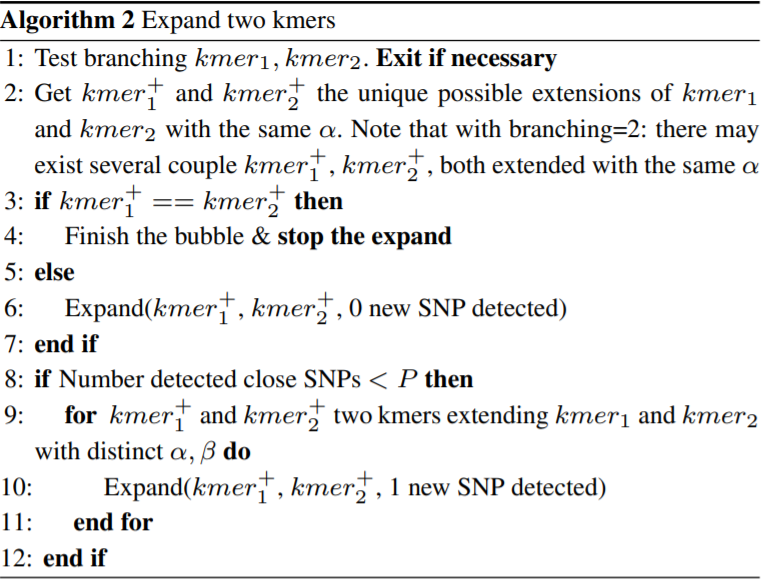
\includegraphics[width=.8\linewidth]{images/discosnp_alg2.png}
  \caption{1b}
  \label{fig:sfig2}
\end{subfigure}
\end{figure}

\begin{figure}[h]
	\centering
  	\captionsetup{justification=centering}
  	%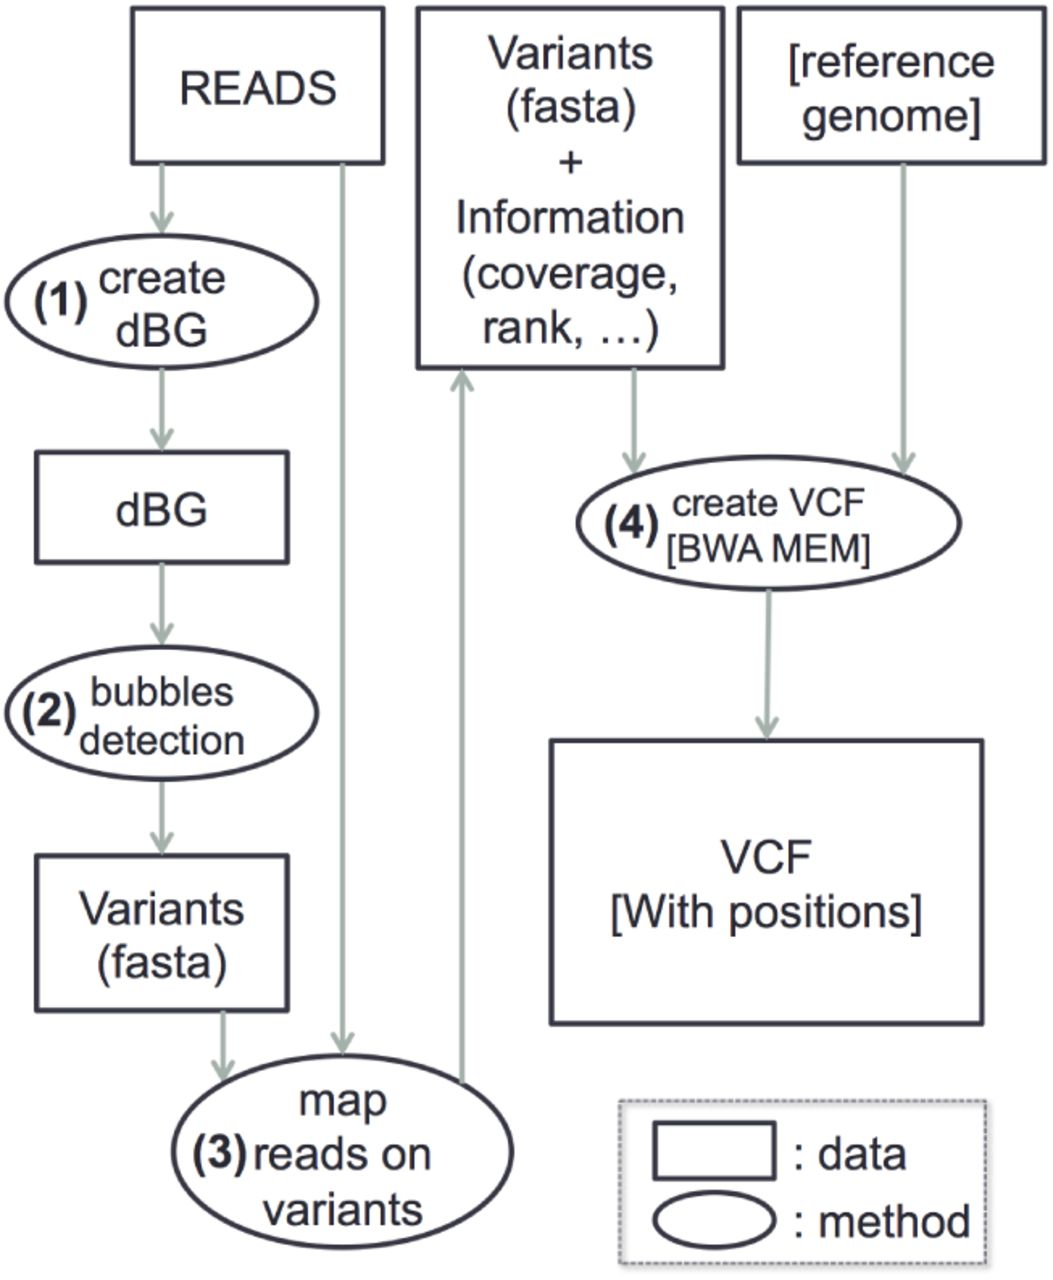
\includegraphics[scale=.90]{images/discosnp_pipeline.jpg}
  	\caption{DiscoSnp\texttt{++} pipeline. Nel caso sia fornito un genoma di riferimento, il VCF file conterrà anche il posizionamento delle previsioni mappate.}
  	\label{fig:pipe1}
\end{figure}

\subsubsection{Prestazioni}




\end{document}
